\color{blue}

\section{Evaluation}

We conducted a pilot user study to evaluate the effectiveness of our approach. 

\subsection{User Study Tasks}

We formulate the following hypotheses to design our user study:

\textbf{H1:} The introduction of rivers can improve the accuracy of locating a CCG in a cartogram.

\textbf{H2:} The introduction of rivers can reduce the time needed to locate a CCG in a cartogram.

\subsection{User Study Variables}

We discuss the variables of our user study in this section.

\subsubsection{Independant Variables}

The primary independent variable is the river-crossing behavior of the nodes, which directly decides the final layout of our cartograms. We set the parameter to either allow or disallow the nodes from crossing a river. The presence of the rivers on the screen is another independent variable. \autoref{table:Independant Variables} shows the combinations we used in our user study.

{
\renewcommand{\arraystretch}{1.5}
\begin{table}[!tb]
	\centering
		\begin{tabulary}{\columnwidth}{|*{2}{c|}}
			\hline
			\cellcolor{Mycolor2}\textbf{River Crossing} &
			\cellcolor{Mycolor2}\textbf{River Presence} \\
			\hline
			Allow & Present \\
			\hline
			Allow & Absent \\
			\hline
			Disallow & Present \\
			\hline
			Disallow & Absent \\
			\hline
		\end{tabulary}
	\caption{The combinations of independent variables.}
	\label{table:Independant Variables}
\end{table}
}


\subsubsection{Dependant Variables}

\bobgraph{Accuracy:} The is the primary dependent variable measured by the number of correct CCGs chosen by the participants.

\bobgraph{Response time:} Another dependant variable is the time taken by the participants to complete each task.

\subsubsection{Control Variables}
\bobgraph{Choice of the color map:} We use D3's built-in interpolateRdYlGn color map, a diverging color scheme of red, yellow, and green, to depict the data in our cartograms.

\bobgraph{Communicating the target CCG to the user:} We inform the participant about the target CCG that they need to find. The target CCG is shown in the form of a non-stop blinking (between its original color and black) area on the screen, each blink is given a duration of 2 seconds.

\subsection{User Study}

\subsubsection{Participants}

We recruited X participants, ...

\subsubsection{Datasets}

We used the following datasets for our evaluation:

\begin{itemize}
    \item Population
    \item Under 75 mortality from cardiovascular disease
    \item Emergency admissions for alcohol-related liver disease
    \item Alcohol-specific admission and readmission
\end{itemize}

135 CGGs are projected on the screen with a choropleth, we then generated another view with our visual design. The color in both visualizations are mapped to population. See \autoref{fig:task}.

{
    \begin{figure}[htb!]
        \centering
        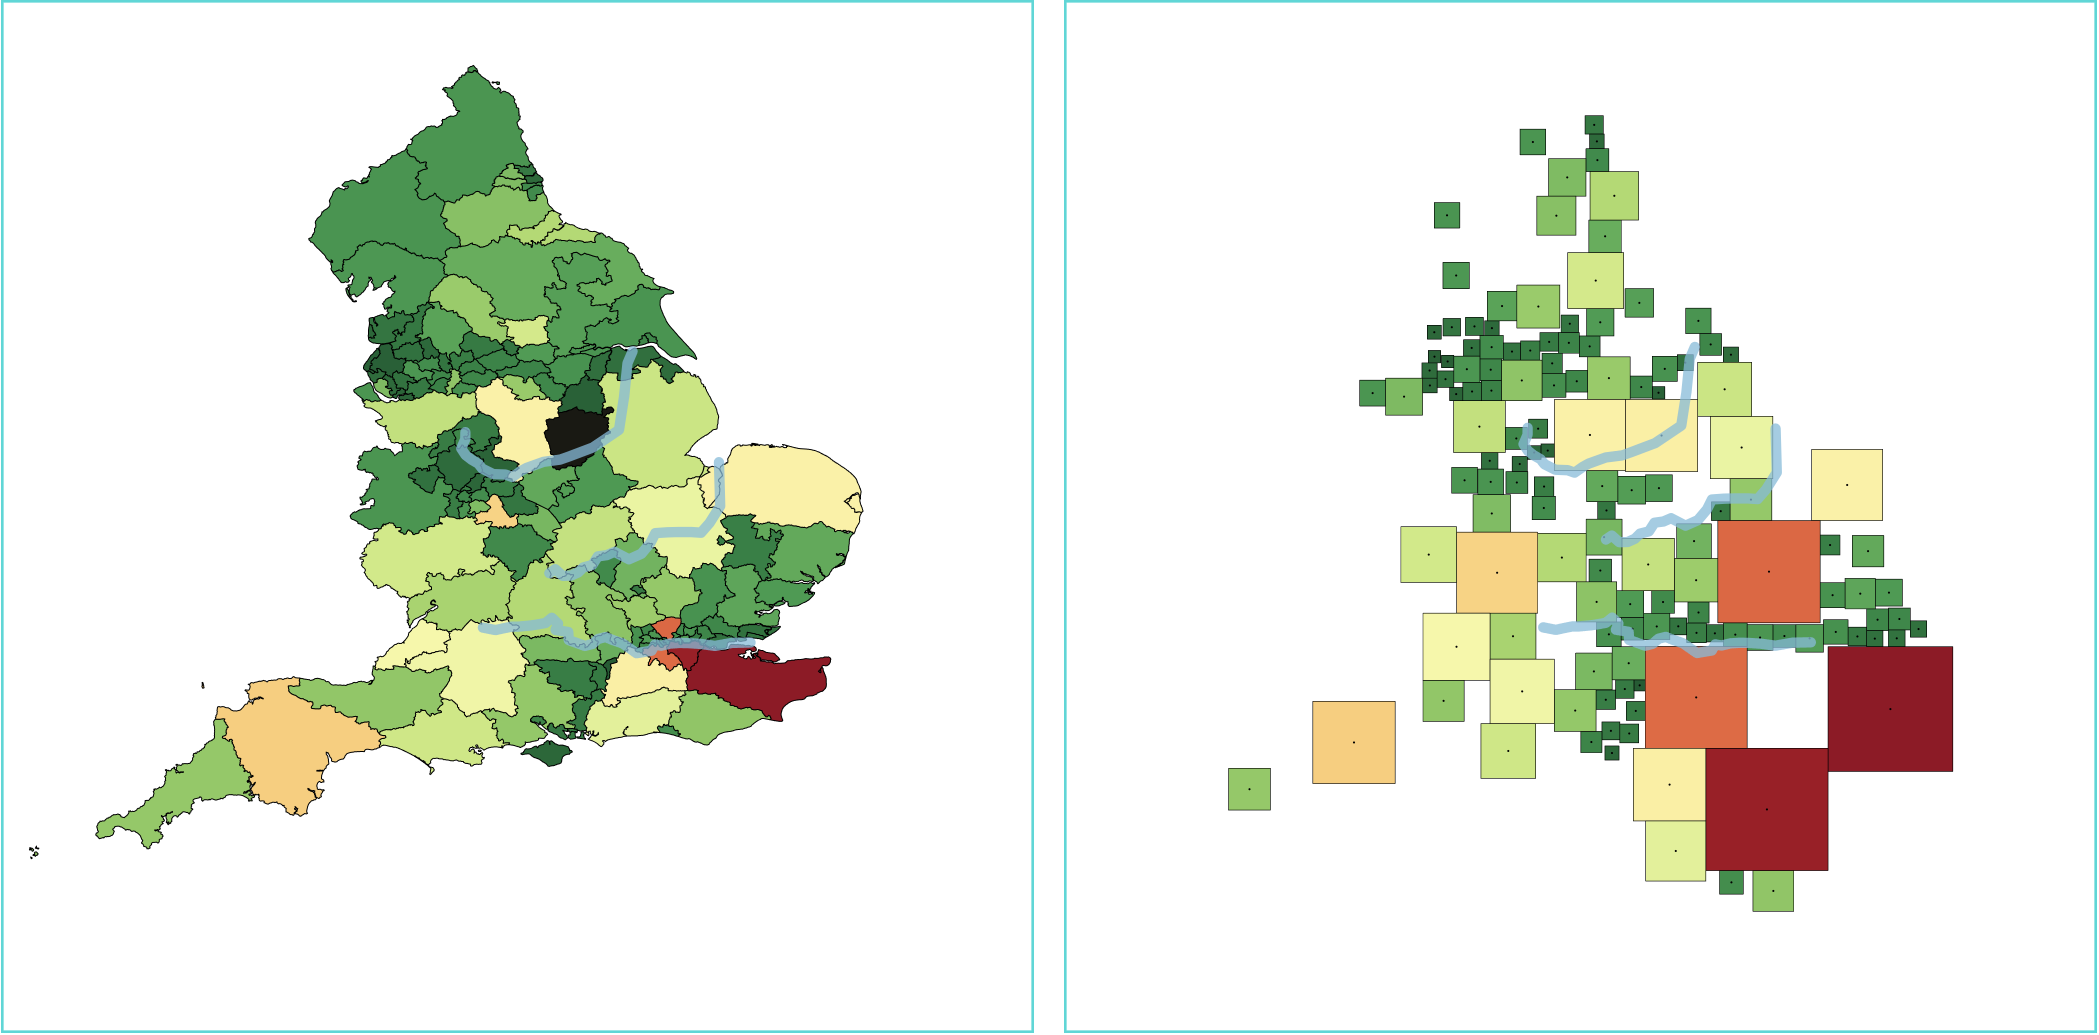
\includegraphics[width=\columnwidth,keepaspectratio]{figure/evaluation/task.png}
        \caption{A typical task for participants. The left shows the choropleth map, and the right shows the cartogram. Both visualizations show the three longest rivers in England, and the color is mapped to CCG population. The target CGG will be blinking on the choropleth (shown in black), participants are asked to identify this CCG on the cartogram.}
        \label{fig:task}
    \end{figure}
}

\subsubsection{Procedure}

The user study was designed to be conducted remotely, and participants were asked to complete the tasks on their own computers. The user study includes four parts:

\textbf{P1:} The participants were asked read instructions and trainings provided in both text and videos. The instructions were designed to help participants understand the concepts used in the tasks. Videos are available at \url{https://www.youtu.be/playlist?list=PLL7sHvxLtD75fMtrUQrAdddjt3wfFkcWz}.

\textbf{P2:} The participants were given three practice tasks to familiarize themselves with the user study. A demonstration of the task is also included in the instructional video.

\textbf{P3:} The participants were asked to complete 16 location tasks. The response and reaction time are recorded. These 16 CCGs were carefully selected to avoid extreme cases (thus biases the result), in terms of size, color, and location.

\textbf{P4:} The participants were asked to complete a questionnaire that consists of Likert Scale questions and open-ended questions.

The user experiment is available at \url{https://osf.io/q39w7}.

\subsection{User Study Results}

\color{black}